\chapter{系統架構與實作}
\label{chapter:system}


\section{實驗平台: free5GC 系統介紹}
\label{sec:free5gc_intro}

% 同時介紹 free5GC control plan 採用 Golang 開發,並且介紹 Golang

free5GC 是一個現行的開源 5G 核心網路方案,在版本 v3.0.4 上原生支援 5G SA (stand-along) 架構,也就是不需要藉由 4G 網路作為中間層,包含核心網路與無線訊號接入端 (RAN, radio access network) 都可以並且必須是純 5G 之架構。而 free5GC 在 v3.0.4 上已經有實作 AMF、AUSF、NRF、NSSF、PCF、SMF、UDM、UDR、與 UPF (見圖~\ref{fig:free5gc_arch}),對於非 3GPP 接入 (non-3gpp access),free5GC 亦有 N3IWF 的支援,是目前開源 5G 核心網路方案中,架構上最爲完善的軟體。由於其開源的性質與廣大的設群討論,基於 free5GC 進行修改開發無疑是最為方便有效之選擇。

\begin{figure}[htbp]
  \centering
  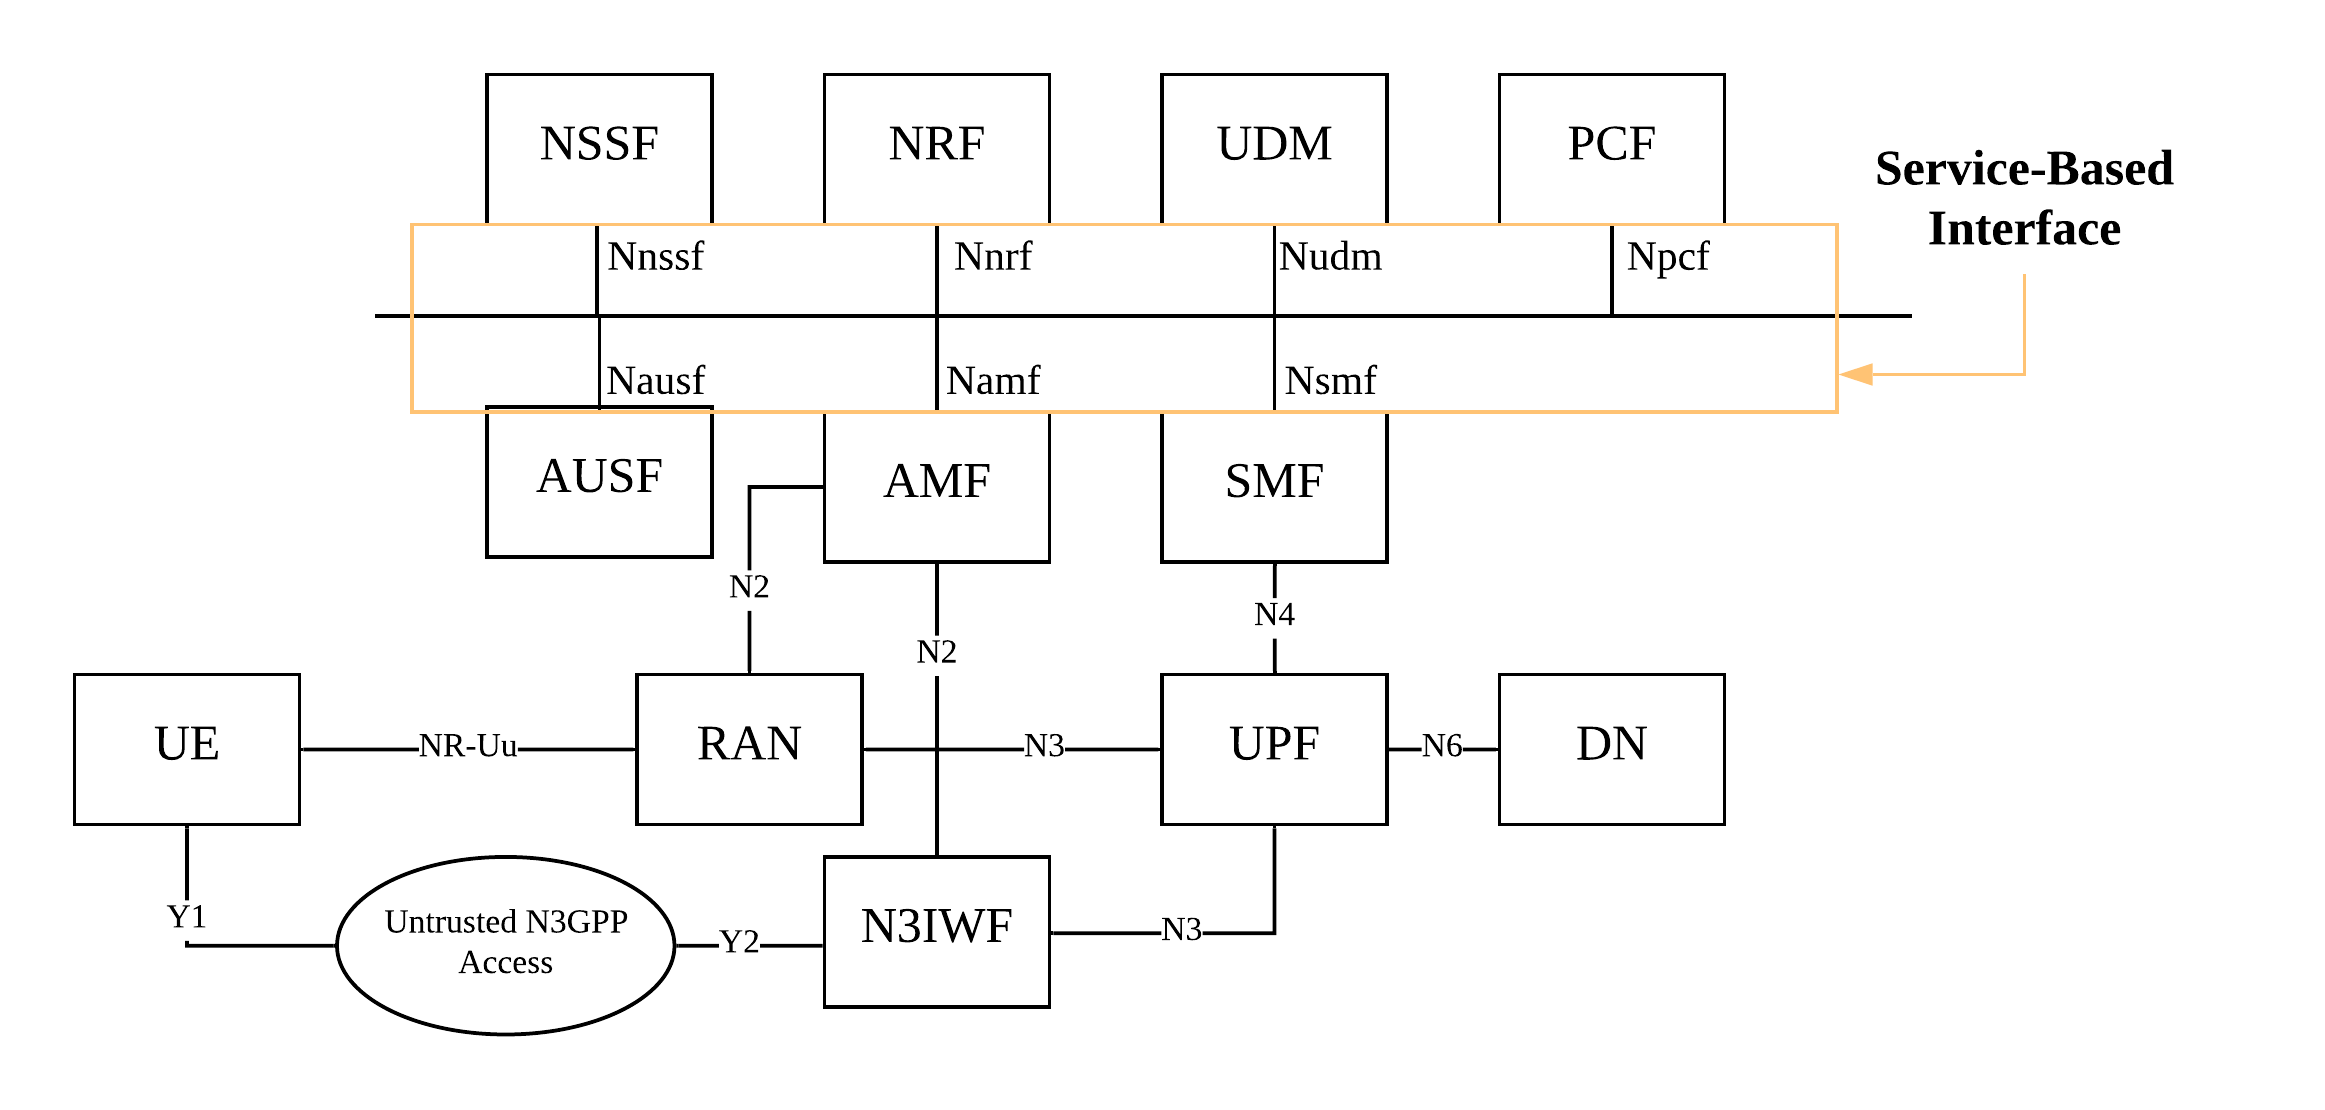
\includegraphics[height=!,width=1\linewidth,keepaspectratio=true]
                    {figures/free5gc-stage-2-arch}
  % [] 放的是顯示在 list of figure 的文字
  % {} 放的是顯示在圖下方的文字
  \caption[free5GC 架構]{{\footnotesize free5GC 架構~\cite{free5gc}}}
  \label{fig:free5gc_arch}
\end{figure}

free5GC 源自於 NextEPC~\cite{nextepc},一個 4G 開源核心網路,於版本 v1.0.0 時將 NextEPC 之 MME、S/P-GW 等運算、管理連線之 NF,改為 5G 之 AMF、SMF、與 UPF,並保留了 4G 的 HSS 與 PCRF 作認證之功能,此階段是對於 5G 架構的概念性驗證 (PoC, Proof of Concept),並沒有完全按照 3GPP 的標準實作。並且由於 NextEPC 是使用 C 語言開發,在此版本下,free5GC 亦是使用 C 語言開發,並且大量繼承使用 NextEPC 之功能與函式。

於版本 v2.0.0 時,free5GC 完全重構了核心網路,捨棄掉 NextEPC 的程式碼而改為重新開發一個基於 3GPP R15.3 的 5G 核心網路。由於考量到 Go 語言有許多適合撰寫網路程式的特性,諸如原生提供大量方便使用之標準函式庫 (standard library)、內建垃圾回收機制 (GC, garbage collection)、可快速引用第三方函式庫 (third party library) 等等,而選擇使用 Go 語言作來撰寫所有控制端 NF,唯獨 UPF 因為考量到效能以及未來可能需要與其他高效能函式庫間接的關係,而沿用 C 語言開發。

% free5GC 原來之 SMF 架構,PFCP 使用 TLV,SBI 使用 HTTP2, OpenAPI
經過了對 free5GC 的程式碼的研讀後,我們瞭解 free5GC 大致上把控制端的 NF 大致規劃成三種部件:SBI、中心處理部件、與其他。以 SMF 為例 (見圖~\ref{fig:free5gc_smf_arch}),分為 SBI、Flow Procedure、與 PFCP。
SBI~\cite{3gpp.29.500} 全名為 service base interface
,是 3GPP 於 R15 (5GS) 設計出來做爲控制端溝通的協定,主要基於 HTTP2、RESTful API 設計,分為 Consumer 與 Producer,由 Consumer 向 Producer 要求 (request) 資訊。相較於 HTTP,HTTP2 提供了更少的網路延遲,而使用 RESTful API 則可讓 API 有更加的結構,並且 3GPP 直接採用 OpenAPI 格式來定義 RESTful 的格式,得以在設計好 OpenAPI 文件後,可讓人類快速讀懂,也可以透過 OpenAPI 工具直接產生出相對應的程式碼,而 free5GC 正是透過 OpenAPI generator 工具把 3GPP 定義的 SBI YAML 檔案轉譯出 Go 語言的 gin server 程式。
PFCP~\cite{3gpp.29.244} 是 SMF 獨有的協議,不存在於除 SMF 與 UPF 外的其他 NF,主要是用來讓 SMF 與 UPF 溝通,並且對 UPF 下達相對應的封包轉發指令,於 3GPP 在 R14 時為了設計 4G EPC 中 CUPS (Control and User Plane Separation, 控制與使用者端分離) 而採用的。PFCP 建立於 UDP 之上並採用 TLV (type, length, value) 的格式設計,封包內容裡每個 IE (information element) 都會有三個主要成分:2 byte 的 type 用來描述 IE 種類、2 byte 的 length 用來描述 IE value 的長度、以及 length byte 的 value 用來敘述 IE 的內容。而 TLV 亦可巢狀使用,及一個 TLV 的 value 內可以包含其他一個或多個 TLV 使用。透過 TLV 的設計,PFCP 可以將訊息有效的壓縮長度。
而 flow procedure 則是負責整個 SMF 的邏輯運算,經過 PFCP 或 SBI 解碼過的內容會被統一傳送給 Flow Procedure 並且由 Flow procedure 來決定相對要做的事情。

其他控制端 NF 架構上大致類似,若是只有 SBI 界面的 NF 像是 UDM、PCF 等等,會捨棄其他部件,而像是 AMF 有 SBI 與 NGAP,則會用 NGAP 取代其他部件。

% free5GC UPF 架構
至於 free5GC 使用者端的 NF UPF 則是主要分成三個部分:N4 Handler、UPDK、與 gtp5g~\cite{gtp5g} (見圖~\ref{fig:free5gc_upf_arch})\cnote{圖尚未補},N4 Handler 主要是負責處理從 SMF 送下來的 PFCP 控制訊號,他會直接透過 Linux UDP Socket 獲取 N4 訊號,解碼 PFCP 後翻譯成 UPF 看得懂的格式,比較有趣的是,因為 PFCP 是遵守 TLV 格式的,因此 free5GC 在撰寫這部分時,是直接解析 3GPP 文件後透過自己撰寫的程式碼生成器 (code generator) 來產生 encoder 與 decoder。UPDK 主要是負責處理使用者端訊息的邏輯,向上他會接收到 N4 Handler 所下的 PDR (Packet Detection Rules) / FAR (Forwarding Action Rules) 指令儲存起來,並在收到相對應的 GTP (GPRS Tunnelling Protocol) 封包後協助 gtp5g kernel module 進行相對應的封包處理。而 gtp5g 則是負責協助處理使用者端界面 N3、N6、與 N9 的 kernel module,在 N6 界面上,會透過 netlink 創造一個虛擬裝置 (virtual device) 來接收從 DN 來的封包,N3 與 N9 則是直接從 netlink module 拿到 routing 進來的封包。

\cnote{圖要崇畫}
\begin{figure}[htbp]
  \centering
  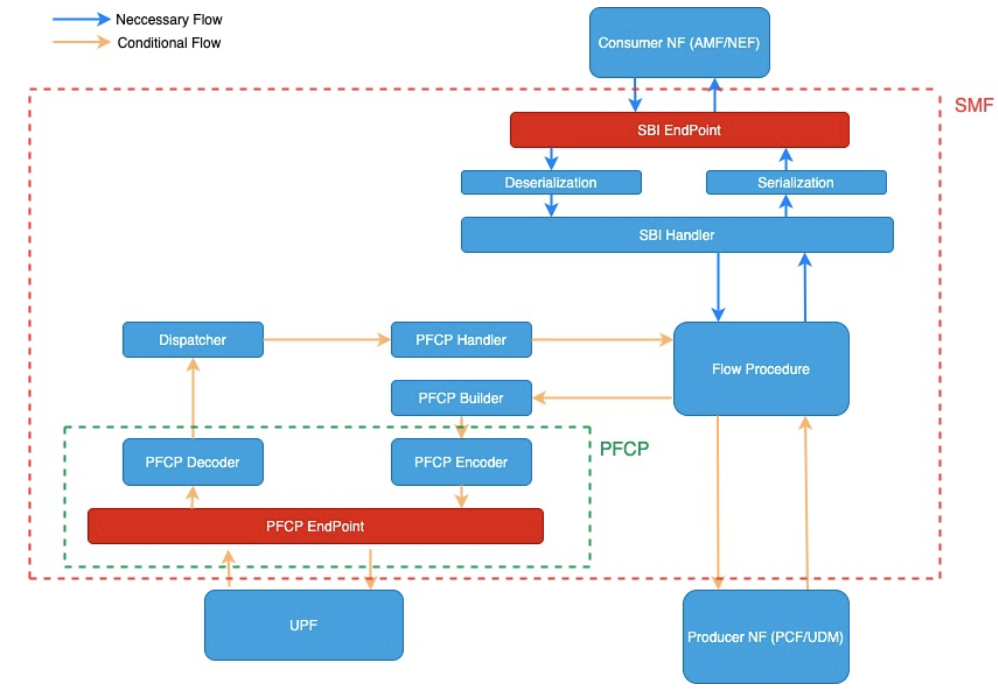
\includegraphics[height=!,width=1\linewidth,keepaspectratio=true]
                  {figures/free5gc_smf_arch}
  % [] 放的是顯示在 list of figure 的文字
  % {} 放的是顯示在圖下方的文字
  \caption[free5GC 原生之 SMF 架構]{{\footnotesize free5GC 原生之 SMF 架構}}
  \label{fig:free5gc_smf_arch}
\end{figure}

\section{系統層 API: OpenNetVM 系統介紹}
\label{sec:opennetvm_intro}

OpenNetVM 是一個由 加利福尼亞大學河濱分校 (UCR) 與 喬治華盛頓大學 (GW) 共同開發,基於 DPDK、Docker 容器、與共享記憶體 (shared memory) 設計的開發平臺,目標在於提供 Network Function 有更好的管理與效能,有幾個主要的優勢:

\begin{itemize}
\item \textbf{Container-based NFs:} OpenNetVM 平臺透過 Docker 容器管理運行於平臺上的 Network Function,因此只需要用一般 user space 程式的撰寫方式開發網路功能便可以輕易部屬至 OpenNetVM 平臺之上。
\item \textbf{NF Manager:} OpenNetVM 平臺透過管理程式 NF Manager 可以持續追蹤平臺上 Network Function 的狀態,並且分配相對應的封包及與 Network Function 內。
\item \textbf{SDN-enabled:} NF Manager 透過 Open Flow 協議向上支援與 SDN 控制器溝通,並可以讓 SDN 控制器組合多個 Network Function 建立服務鏈 (service chain)。
\item \textbf{Zero-Copy IO:} 封包透過直接記憶體存取打入 NF Manager 可以存取的共享記憶體空間中,再由 NF Manager 分配給 Network Function 直接存取封包的能力,過程中無需經過多於的封包複製。
\item \textbf{No Interrupts:} 透過 DPDK 的 polling 模式,封包直接由特定 CPU 固定拉取,而無需透過傳統的中斷 (Interrupt) 處理的方式處理,這可以讓系統在 10Gbps 甚至更高的流量時都還保持著線性的封包處理效能。
\item \textbf{Scalable:} Network Function 可以被輕鬆的複製擴充,NF Manager 會自動對封包作覆載平衡 (load balence) 以提供最大網路效能。
\end{itemize}

% Onvm 架構
\cnote{TODO ONVM architecture}
\begin{figure}[htbp]
    \centering
    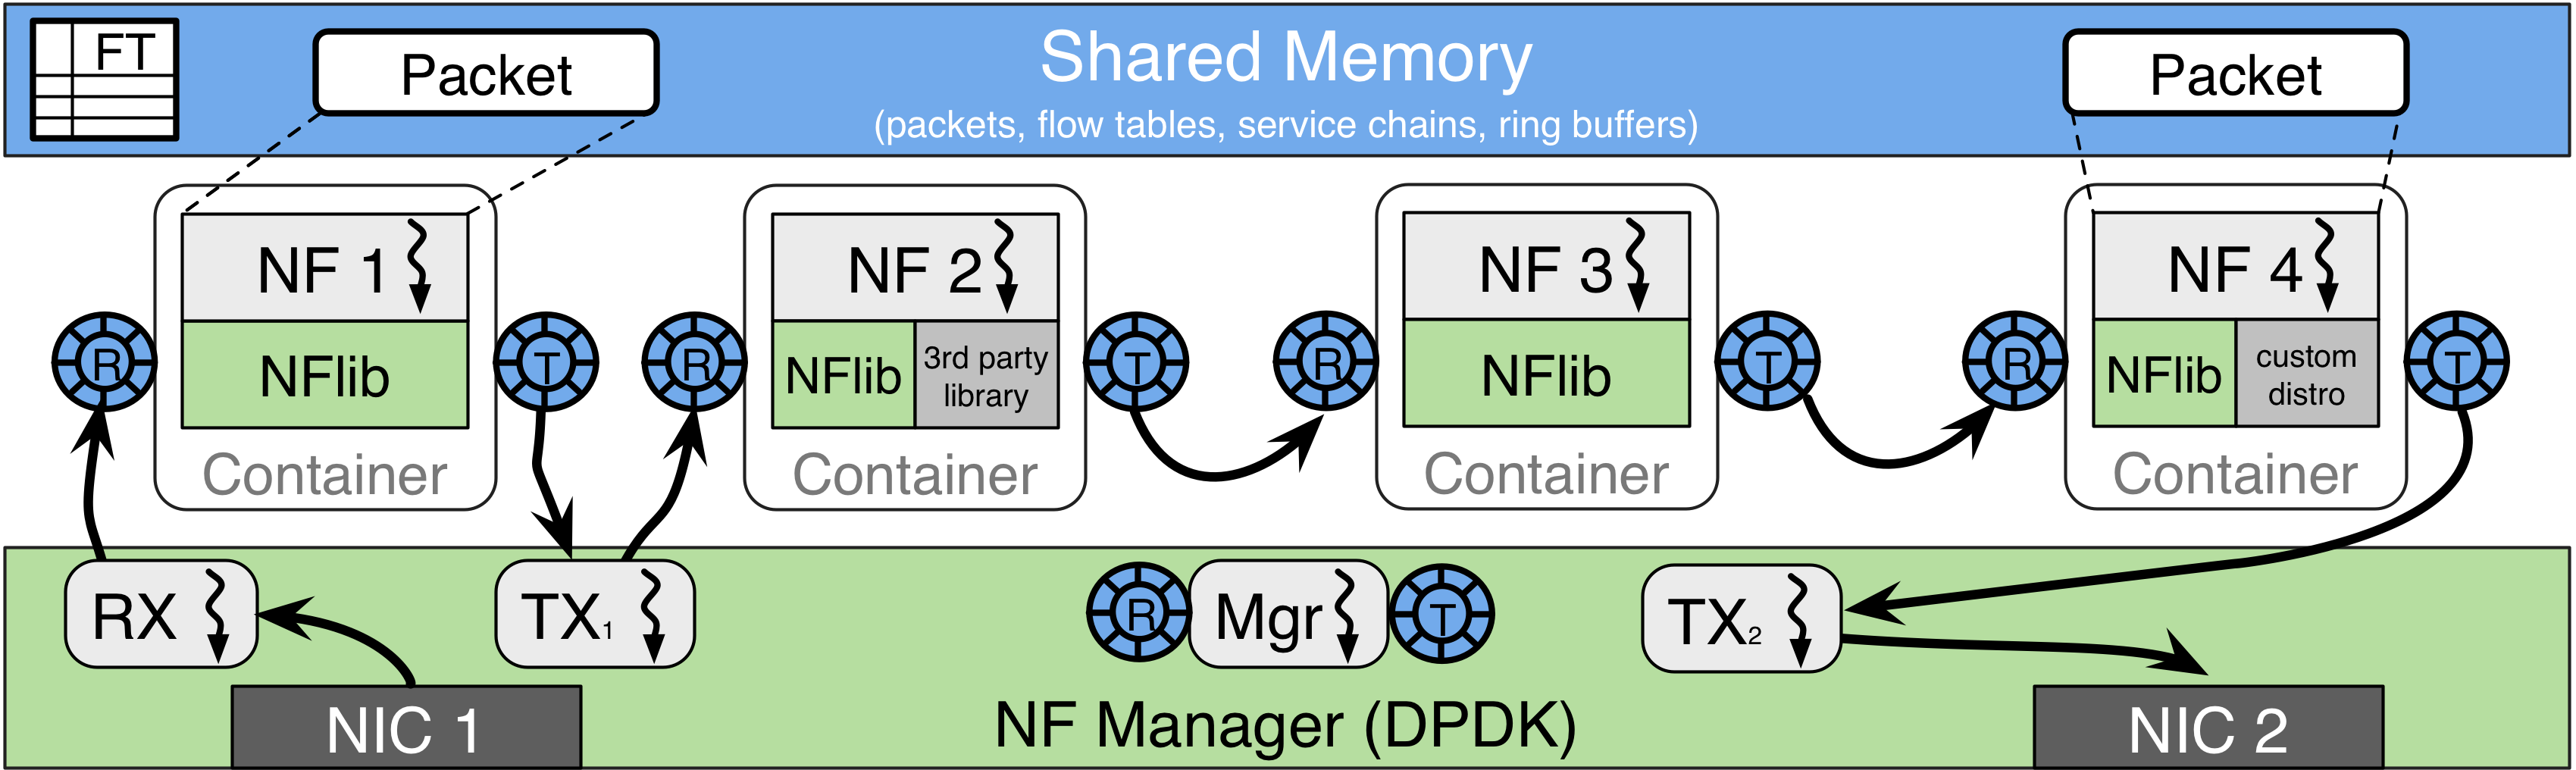
\includegraphics[height=!,width=1\linewidth,keepaspectratio=true]
                    {figures/netvm-arch.png}
                    % [] 放的是顯示在 list of figure 的文字
                    % {} 放的是顯示在圖下方的文字
                    \caption[OpenNetVM 架構]{{\footnotesize OpenNetVM 架構 \cite{onvm}}}
                    \label{fig:netvm_arch}
\end{figure}

% 選擇 ONVM 理由、好處
透過 OpenNetVM 的 API (Application Programming Interface) 設計,我們可以快速開發基於 DPDK 與共享記憶體的網路程式,因此開發 NF 時不需要考慮系統底層實作細節,大大的減少了開發所需時間。另外由於平臺是基於 Docker 容器包裹 NF,因此只需要可以跑在容器內的程式都可以部屬進此平臺內,同時可以享受容器隔離 (isolation) 的安全性,以及快速部屬、擴張的方便性。另外由於有 NF Manager 的幫助,我們無需對 NF 作進一步的管理,只需著重於單一 NF 的開發即可,大幅減少開發時對對管理與部屬所消耗的心力。

\section{系統架構總覽與目標}
\label{sec:arch_intro}
\cnote{TODO}

\section{SMF 移植細節}
\label{sec:smf_porting}

% 5G 所有 interface
雖然 5G 使用 SBI 架構整合了大部分的控制端界面,但還是保留了 NGAP 跟 PFCP 於 N2 及 N4 界面 (見圖~\ref{fig:5g_system_architecture}),其中 N2 是介於基地臺 (RAN) 與 AMF 之間的通訊,透過 NGAP 協定,類似於 4G 時代的 S1AP 協定,而 N4 則是 SMF 與 UPF 間的界面,沿用 4G R10 之後 CU 分離概念所使用的 PFCP 協定。在這主要的三個界面中,SBI 是基於 HTTP2,傳輸層 (L4, transport layer) 是使用的是 TCP,NGAP 的傳輸層使用 SCTP,而 PFCP 的傳輸層使用的是 UDP。

\begin{figure}[ht]
  \centering
  \subcaptionbox[b]{
    5G 系統架構,控制端用 SBI 表示
    \label{fig:5g_system_architecture_sbi}
  }{
    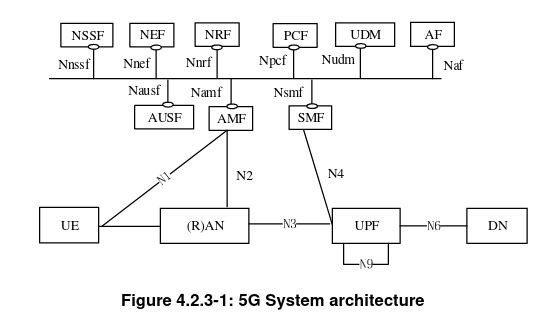
\includegraphics[height=!,width=0.45\linewidth,keepaspectratio=true]
                    {figures/23_501_4-2-3-1_sys_arch_sbi}
  }
  \subcaptionbox[b]{
    5G 系統架構,控制端用參考點表示
    \label{fig:5g_system_architecture_interface}
  }{
    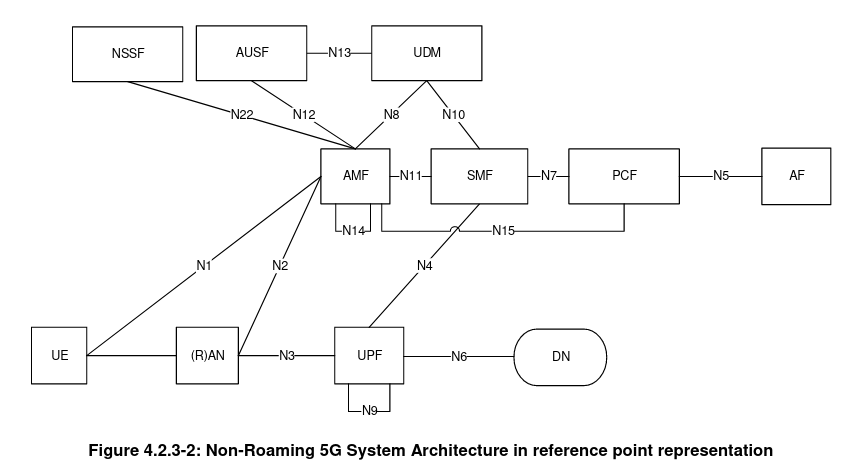
\includegraphics[height=!,width=0.45\linewidth,keepaspectratio=true]
                    {figures/23_501_4-2-3-2_sys_arch_ref}
  }
  % [] 放的是顯示在 list of figure 的文字
  % {} 放的是顯示在圖下方的文字
  \caption[5G 系統架構]{{\footnotesize 5G 系統架構~\cite{3gpp.23.501}}}
  \label{fig:5g_system_architecture}
\end{figure}

% AMF, SMF, UPF 互動內容
由於我們希望專注於改善行動網路最常見的連線行為, UE 連線上網的效能,參與這個情境需要幾乎所有 NF 的參與,但其中有三個 NF 扮演著最重要的角色,AMF、SMF、和 UPF,如同章節~\ref{sec:5g_core_intro}所描述的,AMF 主要負責處理接入 (access) 與移動 (mobility),SMF 負責連線的管理 (session management),而 UPF 則是使用者端 (user plane) 封包最重要且唯一的轉送處理單元。

連線過程主要可以分為兩個階段:註冊 (register) 與連線建立 (Session Establishment)。連線過程會做諸如確認 UE 位置、驗證使用者資料、確認使用者能力、確認一些上下文、或給予 ID 等,主要由 AMF 參與並且向其他 NF (ex. UDM, AUSF) 詢問一些資訊。而連線建立主要會幫助 UE 建立正確的連線路徑、設定 QoS 參數、設定緩衝參數等等,而在這個階段裡,除了 AMF,SMF 與 UPF 也會在這個階段內參與運算,此時 SMF 負責管理與建立連線路徑,向核心網路端他會通知 UPF 建立路徑,而向 RAN 端他會透過 AMF 的中繼 (relay),向 RAN 發出指令建立路徑或詢問資訊。

\begin{figure}[htbp]
  \centering
  \subcaptionbox[b]{
    註冊流程
    \label{fig:reg_proc}
  }{
    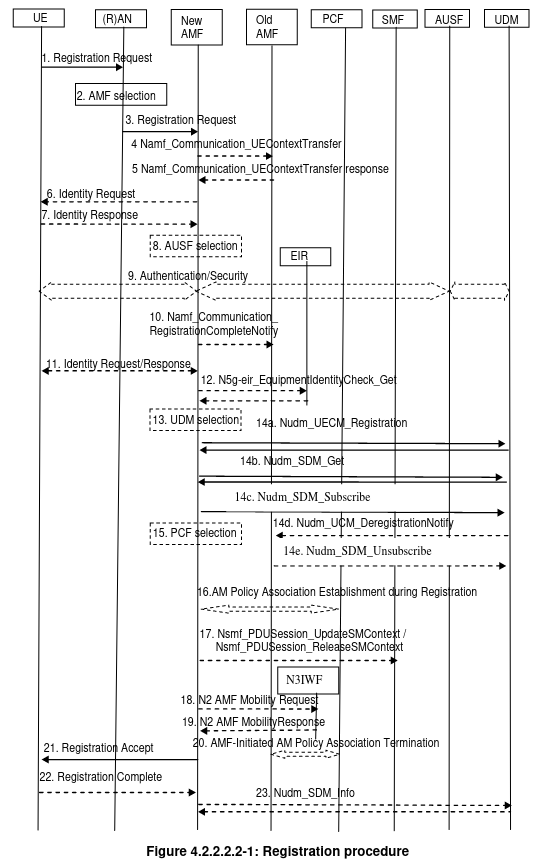
\includegraphics[height=!,width=0.4\linewidth,keepaspectratio=true]
                    {figures/23_502_4_2_2_2_2-1_reg_proc}
  }
  \subcaptionbox[b]{
    連線建立流程
    \label{fig:sess_establish}
  }{
    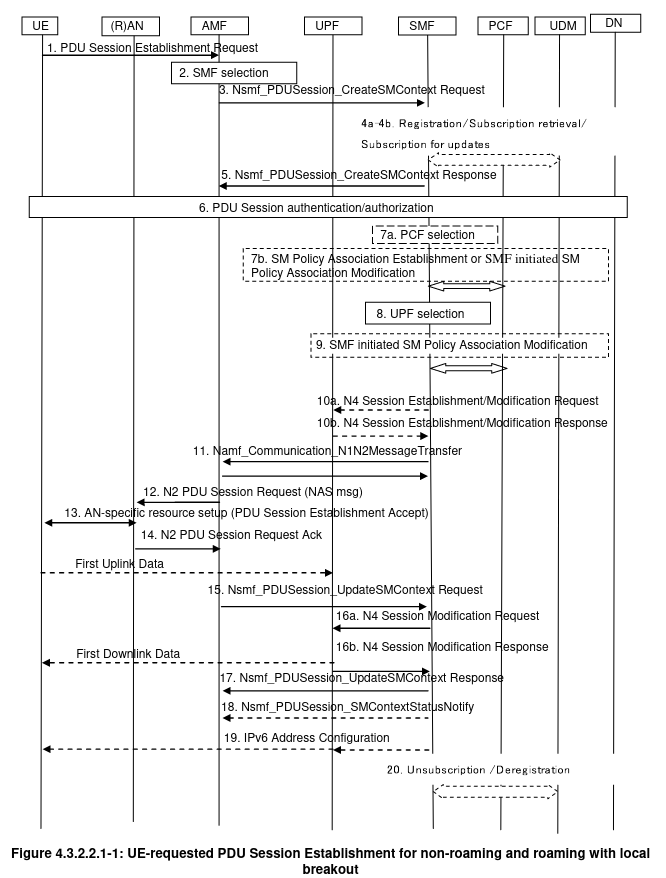
\includegraphics[height=!,width=0.475\linewidth,keepaspectratio=true]
                    {figures/23_502_4_3_2_2_1-1_sess_establish}
  }
  \caption[5G 流程]{{\footnotesize 5G 流程~\cite{3gpp.23.502}}}
  \label{fig:5g_procedure}
\end{figure}


% SMF 所使用的 interface,並且決定只作 PFCP (N4 interface)
% 可以的話舉證 Session mgmt 重要於 mobility 與 regisration/deregistration
為了加速控制端的控制訊號 (control signal) 可以更快的新增、修改、刪除用戶端的會話 (session),我們希望可以透過加速 AMF、SMF、與 UPF 這三個於 PDU Session 流程中最重要的三個 Network Function 之間的通訊速度,降低其三者間的通訊延遲 (latency),得以在 5G 核心網路進行大量會話的新增、修改、與刪除中,得到最好的效能。

在 AMF、SMF、與 UPF 中,SMF 是負責 Session 管理的 Network Function,即是 Session 管理最重要的部件,因此我們希望優先著重於其控制信號的效能最佳化。而在 SMF 的界面中,又以 N4 界面用以對 UPF 下達 Session 管理的界面最為重要,因此我們決定於 N4 界面上,透過 OpenNetVM 物理層傳輸效能的優勢取代傳統 Berkeley Socket,藉以提高 N4 介面的傳輸效能,降低控制訊號的延遲。

% 移植理由, free5GC 目前的 downside (weekness)

原生的 free5GC 控制端界面是建構在 Linux 的 Berkeley Socket 上,先將 L4 層以上的負載內容 (payload) 封裝後,再透過呼叫 Berkeley Socket API,來達成封包傳送的功能。但由於 Berkeley Socket 屬於 user space library API,並且在傳送過程中,至少會經過兩次記憶體複製 (memory copy) (會先複製到 per process 的 kernel space memory,再複製到 network device 的 newtowrk queue) (見圖~\ref{fig:kernel_packet_processing_arch}),相對於後來出現的技術諸如 DPDK 或 XDP,實屬效能不彰。另外,即便是將 Network Function 部屬於同一機器上,由於 Berkeley Socket 屬於 RPC,傳送路徑必定會經過 Network Device,無法自動判定為 IPC 而使用更高效率的傳輸方式。基於以上理由,我們希望透過 OpenNetVM 的性質,同時可以於 RPC 下使用 DPDK 功能,與 IPC 使用 shared memory 功能,實現完全零記憶體複製 (zero copy),以及可於同一主機下使用 IPC 來達到更佳的傳輸效率。除了記憶體複製的問題之外,由於透過 system call 到 kernel 的設計,也會遇到所有 system call 會遇到的問題,像是會有至少兩種中斷 (interrupt),一個是在呼叫 system call 的中斷,另一個則是因為網卡與記憶體是透過 DMA (direct memory access) 的關係,會在 DMA 機制上需要在把封包搬進記憶體後由網卡打入中斷來呼叫中央處理器進行下一步處理。同時 kernel call 也會因為需要上下文切換 (context switch) 到中斷上下文 (interrupt context) 或甚至是遇到程序排程 (process scheduling) 的上下文切換而消耗大量運算資源與效能。

\begin{figure}[htbp]
  \centering
  \begin{tikzpicture}[semithick,scale=1]

    \draw[black, thin] (0,2) -- (16,2);
    \draw[black, thin] (0,5) -- (16,5);

    % Process
    \tikzset{process/.style = {shape=circle,draw,minimum size=1.5em}}
    \node[process] (p) at (8,6.7) {Process};
    % NIC
    \tikzset{NIC/.style = {shape=rectangle,draw,minimum size=1.5em}}
    \node[NIC] (rx) at (5,) {NIC (RX)};
    \node[NIC] (tx) at (11,) {NIC (TX)};
    % Ring
    \coordinate (rx_cod) at (5,3);
    \draw [thin] (rx_cod) circle (0.75);
    \foreach \angle in {90,67.5,...,-67.5}
        \draw ($ (\angle:0.75)+(rx_cod) $) -- ($ (\angle-180:0.75)+(rx_cod) $);
    \node [circle,thick,fill=white,draw=black,align=center] (rx_ring) at (rx_cod) {\tiny RX\\\tiny Ring};
    \coordinate (tx_cod) at (11,3);
    \draw [thin] (tx_cod) circle (0.75);
    \foreach \angle in {90,67.5,...,-67.5}
        \draw ($ (\angle:0.75)+(tx_cod) $) -- ($ (\angle-180:0.75)+(tx_cod) $);
    \node [circle,thick,fill=white,draw=black,align=center] (tx_ring) at (tx_cod) {\tiny TX\\\tiny Ring};
    % buffer
    \tikzset{buff/.style = {shape=rectangle,draw,fill=white,minimum width={width("skb")}}}
    \node[buff] (rx_skb3) at (6.65,3.88) {skb};
    \node[buff] (rx_skb2) at (6.60,3.92) {skb};
    \node[buff] (rx_skb1) at (6.55,3.94) {skb};
    \node[buff] (rx_skb) at (6.5,4) {skb};
    \node[buff] (tx_skb3) at (9.65,3.88) {skb};
    \node[buff] (tx_skb2) at (9.60,3.92) {skb};
    \node[buff] (tx_skb1) at (9.55,3.94) {skb};
    \node[buff] (tx_skb) at (9.5,4) {skb};
    \node[buff] (rx_buf) at (7,6) {recv buff};
    \node[buff] (tx_buf) at (9,6) {send buff};
    % Direction arrow
    \tikzset{copy/.style = {->,> = latex',thick,font=\scriptsize}}
    \draw[copy] (rx) .. controls (6,2) .. (rx_skb) node[pos=0.5] {copy};
    \draw[copy] (rx_skb) -- (rx_buf) node[pos=0.5] {copy};
    \draw[copy] (tx_buf) -- (tx_skb) node[pos=0.5] {copy};
    \draw[copy] (tx_skb) .. controls (10,2) .. (tx) node[pos=0.5] {copy};
    %\draw[copy] (tx_skb) to[out=225,in=135] (tx);
    % DMA & ring buffer
    \draw[double,->,> = latex] (rx) -- (rx_ring) node[pos=0.5] {DMA};
    \draw[double,->,> = latex] (tx_ring) -- (tx) node[pos=0.5] {DMA};
    \draw[dashed,->,thick] (rx_ring) -- (rx_skb);
    \draw[dashed,->,thick] (tx_ring) -- (tx_skb3);
    % text
    \node[text width=3em] at (15,6) {User Space};
    \node[text width=3em] at (15,4) {Kernel Space};
    \node[draw,text width=3em] at (13,5) {Socket};
    \node[draw,text width=3em] at (13,3.7) {Network Stack};
    \node[draw,text width=3em] at (13,2.5) {Driver};
  \end{tikzpicture}

  % [] 放的是顯示在 list of figure 的文字
  % {} 放的是顯示在圖下方的文字
  \caption[核心封包處理架構]{{\footnotesize 核心封包處理架構}}
  \label{fig:kernel_packet_processing_arch}
\end{figure}

不管是控制端界面上的 NGAP、SBI、或 PFCP 都是建立在 Berkely Socket 上,而如章節~\ref{sec:challenge}所述,我們認為 5G 核心網路的 NF 因為網路功能虛擬化 (NFV),因此可以放置於同一主機上。除了 NGAP 是 N2 介面的協定,即基地臺與核心網路的連結,因為基地臺並未虛擬化而是需要佈署在邊緣端,因此我們認爲將包含 SBI 與 PFCP 的協定若可以用更高效率的共享記憶體設計取代 Berkeley Socket,將能大幅提高核心網路控制端的效能。更者,由於 SBI 是建立於 TCP 協定之上,還會遇到諸如 TCP 三方交握或流量控制 (flow control)、擁塞控制 (congestion control) 等機制影響效能,移植至 shared memory 應該能大幅提升效能。

% SMF 的改進

% 開發選擇
在 SMF 移植的設計上,由於 OpenNetVM 所提供的是 C 語言的 API,而 free5GC 的 SMF 所使用的是 Golang 語言開發,因此需要考慮到如何跨語言移植。在設計之初有考慮是否需要透過 IPC 溝通,另外啟動一個 relay 將 SMF 的訊息 (message) 先透過 IPC 傳送到n relay process,再由 relay process 呼叫 OpenNetVM API。但由於發現 Golang 本身有提供 CGO 的功能,透過指定語法可以直接呼叫 C 語言 API,因此我們決定以此方法,減少 IPC 溝通的效能損耗。CGO 提供 C 呼叫 Go 語言函式或是 Go 呼叫 C 語言函式,若是以 C 呼叫 Golang,需要先將 Go 函式庫編譯成 share object library (.so 或 .dll 檔),之後再讓 C 語言透過 share object 的方式呼叫,呼叫過程中由於已經編譯成 object file 並使用 dynimic linking 的方式,是由程式跑起來後 loader 來處理,因此對 caller (C 語言程式) 幾乎沒有任何限制。反之如果是 Golang 呼叫 C 語言函式庫,則會有較多限制,例如 callee 部可以有信號 (signal) 呼叫 (基於 golang 本身訊號覆蓋(signal mask)機制)、部分型別需要做強型別轉換、需要透過 cgo flag 讓編譯器或連結器得到相對 library 絕對位置等等。

儘管透過 C program 呼叫 Golang shared library 在實踐成本上遠低於使用 Golang 呼叫 C library,但我們希望在程式設計上可以提供更高的擴充性 (scalibility) 與更加一般化 (generalize),且若可以設計成 函式庫 (library) 形式,會更加利於使用者使用且可以不僅限此專案使用,因此我們希望嘗試以可以直接使用之 Golang 函式庫方向開發。

由於從 OpenNetVM API 上獲取的封包是直接傳回封包所在記憶體位置的指標,而封包爲連結層 (link layer) 之上的內容,因此我們決定開發成類似 Goalng 原生之 net 函式庫,透過 Golang 所提供的 interface 性質,直接取代掉 PFCP 底層之 \lstinline[language=Go]{net.UdpConn} interface,我們命名之 \lstinline[language=Go]{onvmNet.ONVMConn} interface~\cite{github.onvmNet} (見圖~\ref{fig:smf_porting_arch})。

\begin{figure}[htbp]
  \centering
  \subcaptionbox{
    原生之 free5GC SMF 架構
    \label{fig:kernel_smf_arch}
  }{
    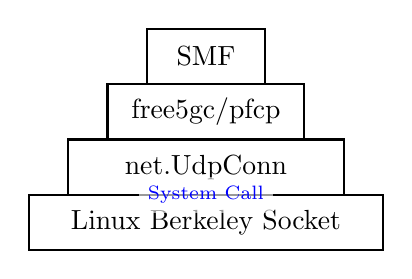
\begin{tikzpicture}
      \tikzset{
        disc 1/.style={minimum width=15mm},
        disc 2/.style={minimum width=25mm},
        disc 3/.style={minimum width=35mm},
        disc 4/.style={minimum width=45mm},
      };
      \tikzset{box/.style={minimum height=2em,draw=black,inner sep=0,thick,node distance=2em}}
      \node[disc 1,draw,box] (d1) {SMF};
      \node[disc 2,draw,box,below of=d1] (d2) {free5gc/pfcp};
      \node[disc 3,draw,box,below of=d2] (d3) {net.UdpConn};
      \node[disc 4,draw,box,below of=d3] (d4) {Linux Berkeley Socket};
      \node[below of=d3,node distance=1em,opacity=0.6,fill=white,text opacity=1,text=blue] {\scriptsize System Call};
    \end{tikzpicture}
  }
  \subcaptionbox{
    OpenNetVM 移植後之 SMF 架構
    \label{fig:onvm_smf_arch}
  }{
    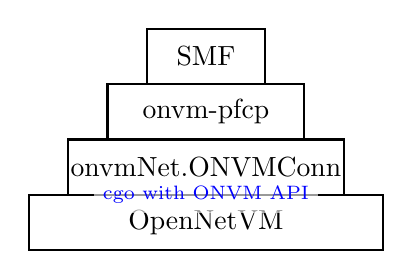
\begin{tikzpicture}
      \tikzset{
        disc 1/.style={minimum width=15mm},
        disc 2/.style={minimum width=25mm},
        disc 3/.style={minimum width=35mm},
        disc 4/.style={minimum width=45mm},
      };
      \tikzset{box/.style={minimum height=2em,draw=black,inner sep=0,thick,node distance=2em}}
      \node[disc 1,draw,box] (d1) {SMF};
      \node[disc 2,draw,box,below of=d1] (d2) {onvm-pfcp};
      \node[disc 3,draw,box,below of=d2] (d3) {onvmNet.ONVMConn};
      \node[disc 4,draw,box,below of=d3] (d4) {OpenNetVM};
      \node[below of=d3,node distance=1em,opacity=0.6,fill=white,text opacity=1,text=blue] {\scriptsize cgo with ONVM API};
    \end{tikzpicture}
  }
  % [] 放的是顯示在 list of figure 的文字
  % {} 放的是顯示在圖下方的文字
  \caption[SMF 相關性依賴]{{\footnotesize SMF 相關性依賴}}
  \label{fig:smf_porting_arch}
\end{figure}

在設計此函式庫時有部分條件需要考慮,首先,由於 Golang 在透過 CGO 呼叫 C 函式時,有不可呼叫內部有訊號註冊 (signal handling) 的函式,其原因爲 Golang 本身有對訊號作內部處理,因此如果透過外部語言另外註冊訊號,會影響 Golang 程序底層訊號處理,但由於 OpenNetVM 在初始化階段需要透過 OpenNetVM 的 API 對系統作訊號註冊,因此會出現問題。而我們參考了網路上的解決方法,將訊號註冊放置 Golang 的 \lstinline[language=Go]{init} 函式,\lstinline[language=Go]{init} 函式是 Golang 設計給予在 main 函式執行起來前,就預先執行的函式,類似 C 語言的 \lstinline[language=C]{__attribute__ ((constructor))}。

然而,使用 \lstinline[language=Go]{init} 函式會遇到初始化參數無法透過程式執行過程中傳遞,因此我們採用 OpenNetVM 提供的 NF config 設計,透過 config 檔預先傳入 OpenNetVM 平臺之必要參數,諸如 DPDK 參數、Service ID、Instence ID 等。

又因為 OpenNetVM 是使用 Service ID 來決定封包目的地應該傳送至那一個 Network Function,而非使用傳統的 IP 來做 routing,因此我們也對應設計了 ipid.yaml 的檔案預先定義 IP 與 Service ID 的對應關係。透過這樣的設計,函式呼叫者 (caller) 可以直接沿用傳統 TCP 或 UDP 的呼叫,進入 onvmNet 函式之後才會透過此 ipid.yaml 檔案映射到相對應的 Service ID。

在方法 (method) 的設計上,因為我們需要繼承 \lstinline[language=Go]{net.Conn} 這個 interface,因此我們實作了此 interface 所有提供之 method,讓使用者得以直接呼叫。

另外在設計封包收取 (ReceiveFrom) 時,需要判斷此封包屬於那一個連線 (connection) 的,因此我們設計了 \lstinline{channelMap},每個連線在聽到 (listen) 連線時會開出一個對應的 channel 並放入 channelMap,當處理者 (handler) 收到 OpenNetVM 給予的封包後,透過 HashMap 的方式以 O(1) 的速度搜尋出相對應的 channel,再將封包送入 channel 得以送到正確的連線中。

\cnote{補 Channel dispacher 設計圖}

設計完 onvmNet 函式庫後,之需將 free5GC 內部 PFCP 函式庫內有呼叫到 \lstinline[language=Go]{net.UDPConn} 的部分改成呼叫 \lstinline[language=Go]{onvmNet.ONVMConn}。另外由於 free5GC 是透過 go module 來維護套件,因此還需跟新 go.mod 之內容。而若有其他 Golang 專案想要嘗試使用 OpenNetVM 平臺,僅需作相同的取代,即可快速移植 (見圖~\ref{fig:free5gc_smf_arch})。

% ONVM SMF 總架構圖
\begin{comment}
\begin{figure}[htbp]
  \centering
  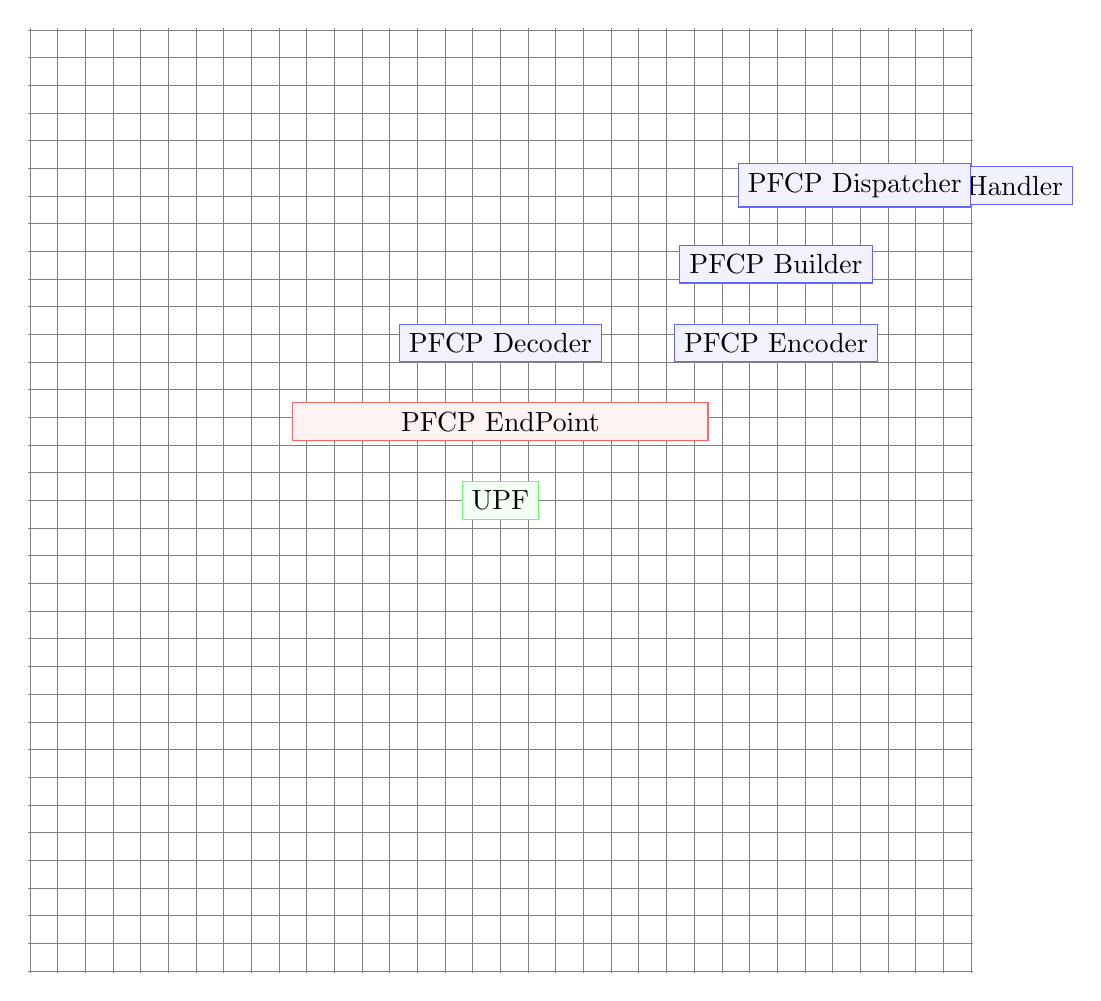
\begin{tikzpicture}
    \draw[step=1em,gray,very thin] (-6,-6) grid (6,6);
    \filldraw[black] (0,0) circle (2pt) node[anchor=west] {};

    \tikzset{
      component/.style={rectangle,draw=blue!60,fill=blue!5,thin,minimum width=7em},
      endpoint/.style={rectangle,draw=red!60,fill=red!5,thin,minimum width=15em},
      nf/.style={rectangle,draw=green!60,fill=green!5,thin},
    };
    \node[nf] (upf) {UPF};
    \node[endpoint] (pfcp_ep) [above of=upf] {PFCP EndPoint};
    \node[component] (pfcp_de) [above of=pfcp_ep] {PFCP Decoder};
    \node[component] (pfcp_en) [above of=pfcp_ep,right of=pfcp_ep,xshift=2.5cm] {PFCP Encoder};
    \node[component] (pfcp_b) [above of=pfcp_en] {PFCP Builder};
    \node[component] (pfcp_han) [above of=pfcp_b,xshift=2.5cm] {PFCP Handler};
    \node[component] (pfcp_dis) [right of=pfcp_han,xshift=-2.5cm] {PFCP Dispatcher};
  \end{tikzpicture}
\end{figure}
\end{comment}

\section{UPF 移植細節}
\label{sec:upf_porting}
\cnote{不確定要不要描述 UPF 部分的細節}
